\documentclass[11pt]{standalone}
\usepackage[dvipsnames]{xcolor}
\usepackage{tikz}
\usepackage{enumitem}

\usepackage{fontspec}
\setmainfont{tex gyre schola}

\begin{document}
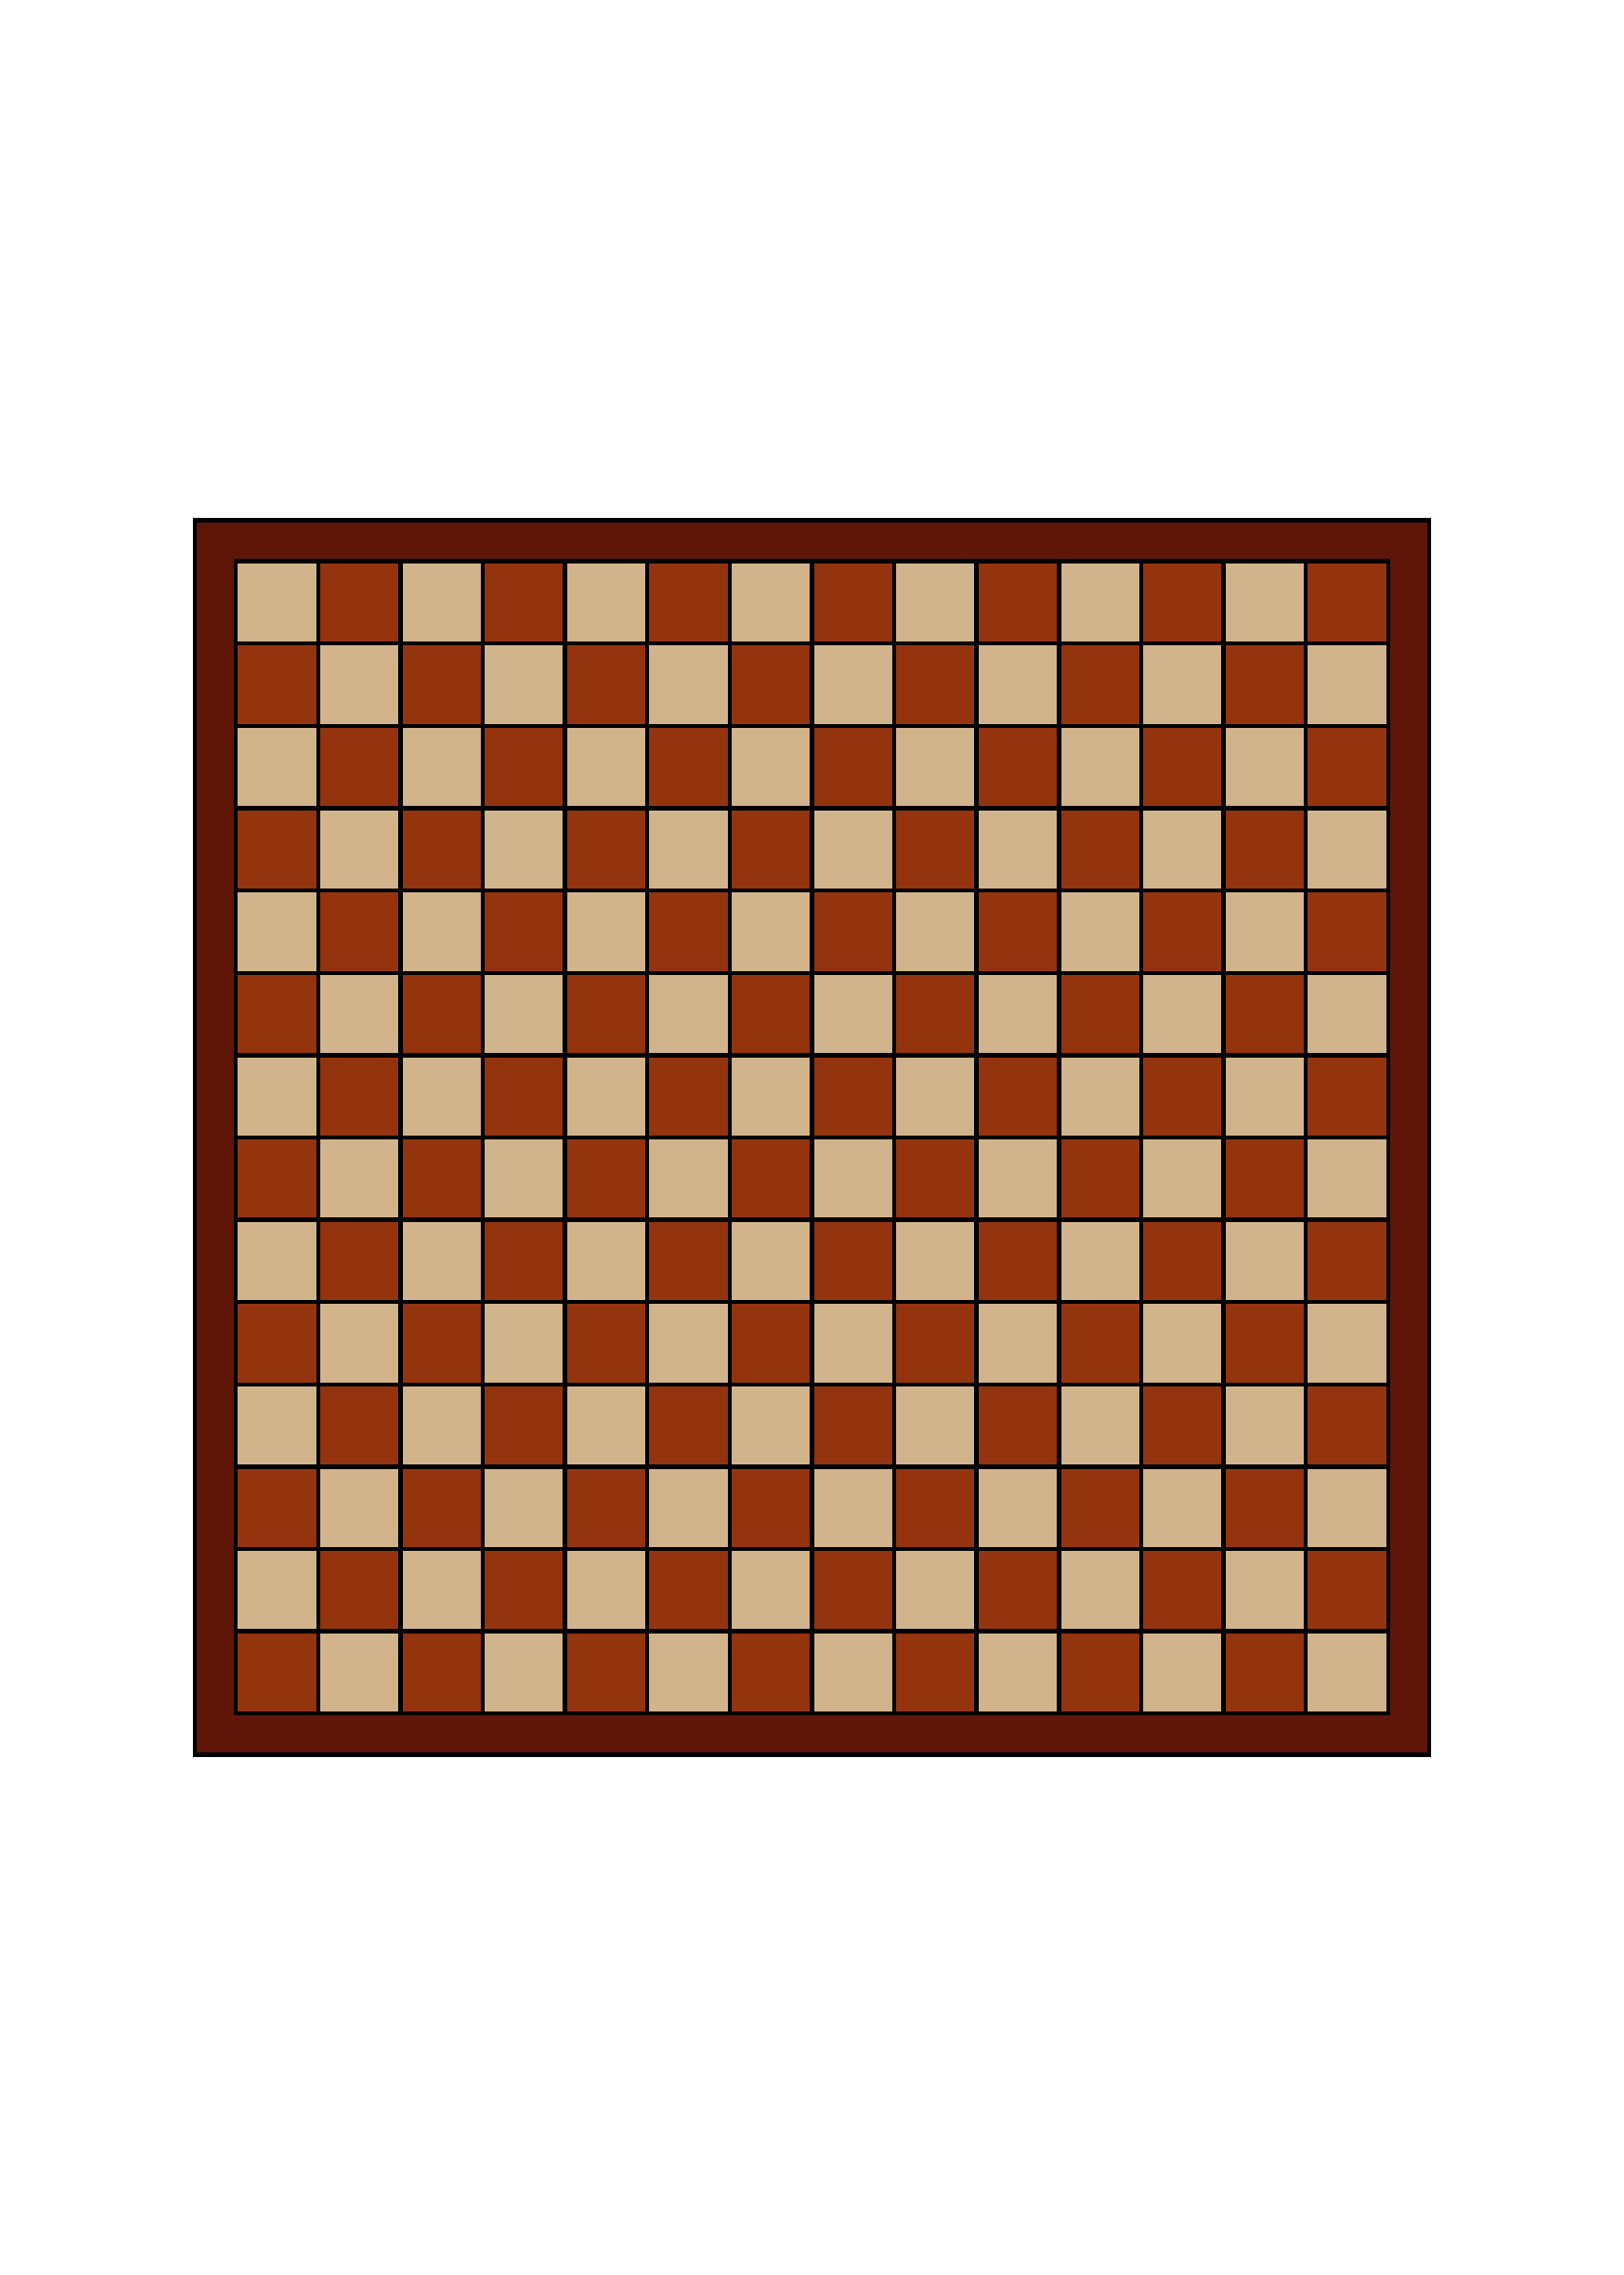
\begin{tikzpicture}
\path (-105mm, -148.5mm) -- (105mm,148.5mm);

\node[draw, ultra thick, fill=Sepia, minimum width=165mm, minimum height=165mm] at (0,0) {};
\node[draw, ultra thick, fill=Tan, minimum width=154mm, minimum height=154mm] at (0,0) {};

\foreach \i in {-6.5, -4.5, -2.5, -0.5, 1.5, 3.5, 5.5}
\foreach \j in {-6.5, -4.5, -2.5, -0.5, 1.5, 3.5, 5.5}
	\node[minimum width=11mm, minimum height=11mm, draw, ultra thick, fill=RawSienna] at (\i*11mm, \j*11mm) {};
	
\foreach \i in {-5.5, -3.5, -1.5, 0.5, 2.5, 4.5, 6.5}
\foreach \j in {-5.5, -3.5, -1.5, 0.5, 2.5, 4.5, 6.5}
	\node[minimum width=11mm, minimum height=11mm, draw, ultra thick, fill=RawSienna] at (\i*11mm, \j*11mm) {};

\end{tikzpicture}
\end{document}